 \documentclass[a4paper,12pt]{article}
\usepackage[a4paper,top=1.3cm,bottom=2cm,left=1.5cm,right=1.5cm,marginparwidth=0.75cm]{geometry}
\usepackage{setspace}
\usepackage{cmap}					
\usepackage{mathtext} 				
\usepackage[T2A]{fontenc}			
\usepackage[utf8]{inputenc}			
\usepackage[english,russian]{babel}
\usepackage{multirow}
\usepackage{graphicx}
\usepackage{wrapfig}
\usepackage{tabularx}
\usepackage{float}
\usepackage{longtable}
\usepackage{hyperref}
\hypersetup{colorlinks=true,urlcolor=blue}
\usepackage[rgb]{xcolor}
\usepackage{amsmath,amsfonts,amssymb,amsthm,mathtools} 
\usepackage{icomma} 
\mathtoolsset{showonlyrefs=true}
\usepackage{euscript}
\usepackage{mathrsfs}

\DeclareMathOperator{\sgn}{\mathop{sgn}}
\newcommand*{\hm}[1]{#1\nobreak\discretionary{}
	{\hbox{$\mathsurround=0pt #1$}}{}}


\title{\textbf{1.4.5 Изучение колебаний струны}}
\author{Платонов Егор}
\date{\today}


\begin{document}
	
	\maketitle
	
	\section{Введение}
	
	\textbf{Цели работы:} изучение поперечных стоячих волн на струне; определение собственных частот колебаний струны; исследование зависимости скорости распространения поперечных волн на струне в зависимости от её натяжения.\\
	\textbf{Оборудование:} закрепленная на станине стальная струна, набор грузов,
	электромагнитные датчики, звуковой генератор, двухканальный осциллограф, частотомер.
	
	\section{Теоретические сведения}
	
	Основное свойство струны -- гибкость, является следствием ее большой длины по сравнению с поперечными размерами. Даже струны, изготовленные из жестких материалов, практически не сопротивляются изгибанию, если размер изгибаемого участка значительно больше поперечного размера струны. Данный факт позволяет не учитывать при дальнейшей работе изгибные напряжения.
	
	Горизонтально закрепленная струна провисает под действием поля тяжести, при отсутствии натяжения. Достаточно натянутую струну можно считать прямой, если ее концы закреплены на одном горизонтальном уровне. Учитывая этот факт, в дальнейшем действие силы тяжести учитываться не будет.
	
	Натянутая струна с жестко закрепленными концами удобна для изучения колебаний. Это связанно с тем, что в струне можно непосредственно наблюдать простейшие типы колебаний и волн, измерять их параметры и сравнивать результаты наблюдения с результатами теоретических расчетов.
	
	Движение элементов струны может быть вызвано изменением ее формы или передачей ей импульса. Натяжение струны стремиться вернуть ее в изначальное прямолинейное положение, и это приводит к тому, что возникает движение элементов струны. Возмущения бегут вдоль струны.
	
	Скорость распространения подобного возмущения можно вычислить по формуле \eqref{velocity_of_deformation}.
	
	\begin{equation}
		u = \sqrt{\frac{T}{\rho_l}}
		\label{velocity_of_deformation}
	\end{equation}
	где $F$ -- сила натяжения струны, $\rho_{l}$ -- масса струны на единицу длины.
	
	При заданной частоте $\nu$ длина волны определяется по формуле:
	
	\begin{equation}
		\lambda = \frac{u}{\nu}
	\end{equation}
	
	Частоты собственных колебаний струны определяются формулой:
	
	\begin{equation}
		\nu_{n} = \frac{nu}{2l} = \frac{n}{2l}\sqrt{\frac{T}{\rho_l}}
		\label{frequency_velocity_equation}
	\end{equation}
	где $n$ -- число полуволн, $l$ -- длина струны.
	
	\section{Экспериментальная установка}
	
	\begin{figure}[h!]
		\begin{center}
			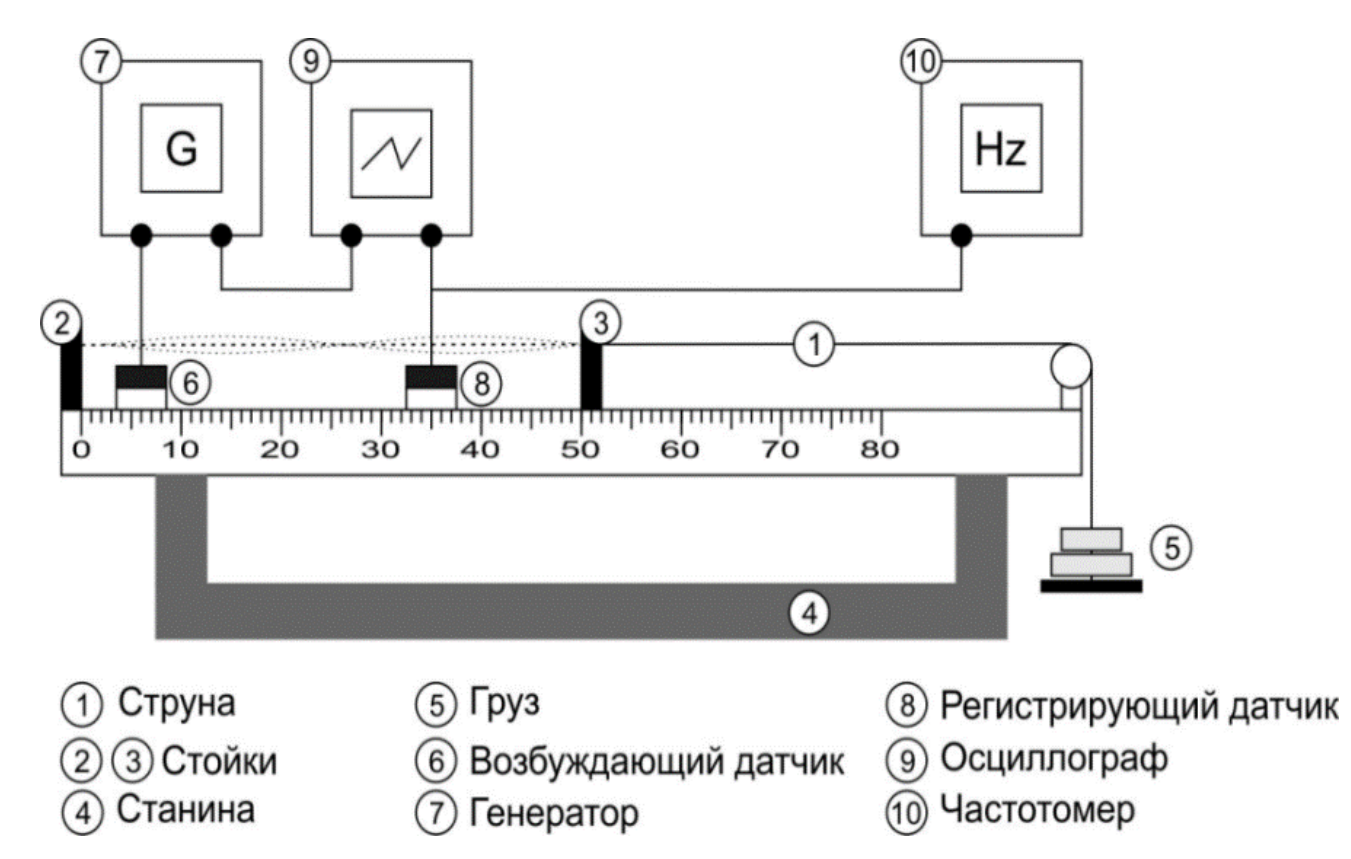
\includegraphics[width = 0.9\textwidth]{Screenshot 2023-10-04 133410.png}
			\caption{Схема экспериментальной установки}
			\label{facility}
		\end{center}
	\end{figure}
	
	Схема установки приведена на рис. 1. Стальная гитарная струна 1 закрепляется в горизонтальном положении между двумя стойками с зажимами 2 и 3, расположенными на массивной станине 4. Один конец струны 
закреплен в зажиме 2 неподвижно. К противоположному концу струны, перекинутому через блок, прикреплена платформа с грузами 5, создающими 
натяжение струны. Зажим 3 можно передвигать по станине, устанавливая 
требуемую длину струны. Возбуждение и регистрация колебаний струны 
осуществляются с помощью электромагнитных датчиков (вибраторов), 
расположенных на станине под струной. Электромагнитный датчик 6 подключен к звуковому генератору 7 и служит для возбуждения колебаний струны, частота которых измеряется с помощью частотомера 10 (в некоторых установках частотомер встроен в генератор). Колебания струны регистрируются с помощью электромагнитного датчика 8, сигнал с которого 
передается на вход осциллографа 9. Разъёмы, через которые датчики с помощью кабелей соединяются с генератором и осциллографом, расположены на корпусе станины.
\pagebreak

\section{Результаты измерений и обработка данных}

Для создания различных сил натяжения струны были использованы грузы, массы которых представлены в таблице 1.

\begin{table}[!ht]
    \caption{Используемые массы грузов (с учетом массы подвеса)}
    \centering
    \begin{tabular}{|l|l|l|l|l|}
    \hline
        $m_1$, г & $m_2$, г & $m_3$, г & $m_4$, г & $m_5$, г \\ \hline
        1106 & 1440,3 & 1927,2 & 2087,9 & 2422,2 \\ \hline
    \end{tabular}
\end{table}

Силы натяжения вычислены по формуле $T_i = m_ig$, где $g=9,8$  $\frac{\text{м}}{\text{с}^2}$

 \begin{table}[!ht]
    \caption{Результаты измерений $\nu_n$ для 5 гармоник для разных сил натяжения}
    \centering
    \begin{tabular}{|l|l|l|l|l|l|}
    \hline
        T, H & $\nu_1$ & $\nu_2$ & $\nu_3$ & $\nu_4$ & $\nu_5$ \\ \hline
        10,84 & 137,4 & 277 & 416 & 557 & 695 \\ \hline
        14,11 & 155,3 & 312,2 & 468,3 & 626,5 & 782,6 \\ \hline
        18,89 & 179,4 & 360,3 & 540,1 & 721,7 & 902,1 \\ \hline
        20,46 & 186,6 & 374,1 & 561,9 & 751 & 938,3 \\ \hline
        23,74 & 200,9 & 403,1 & 605,4 & 807,7 & 1010,1 \\ \hline
    \end{tabular}
\end{table}
По данным из таблицы 2 построен график зависимости частоты $\nu_n$ от номера гармоники $n$ для разных сил натяжения (рис. 2). С помощью МНК проведена линейная аппроксимация зависимости. На графике больший угол наклона аппроксимирующей прямой соответствует большей силе натяжения нити.

\begin{figure}[h]
    \centering
    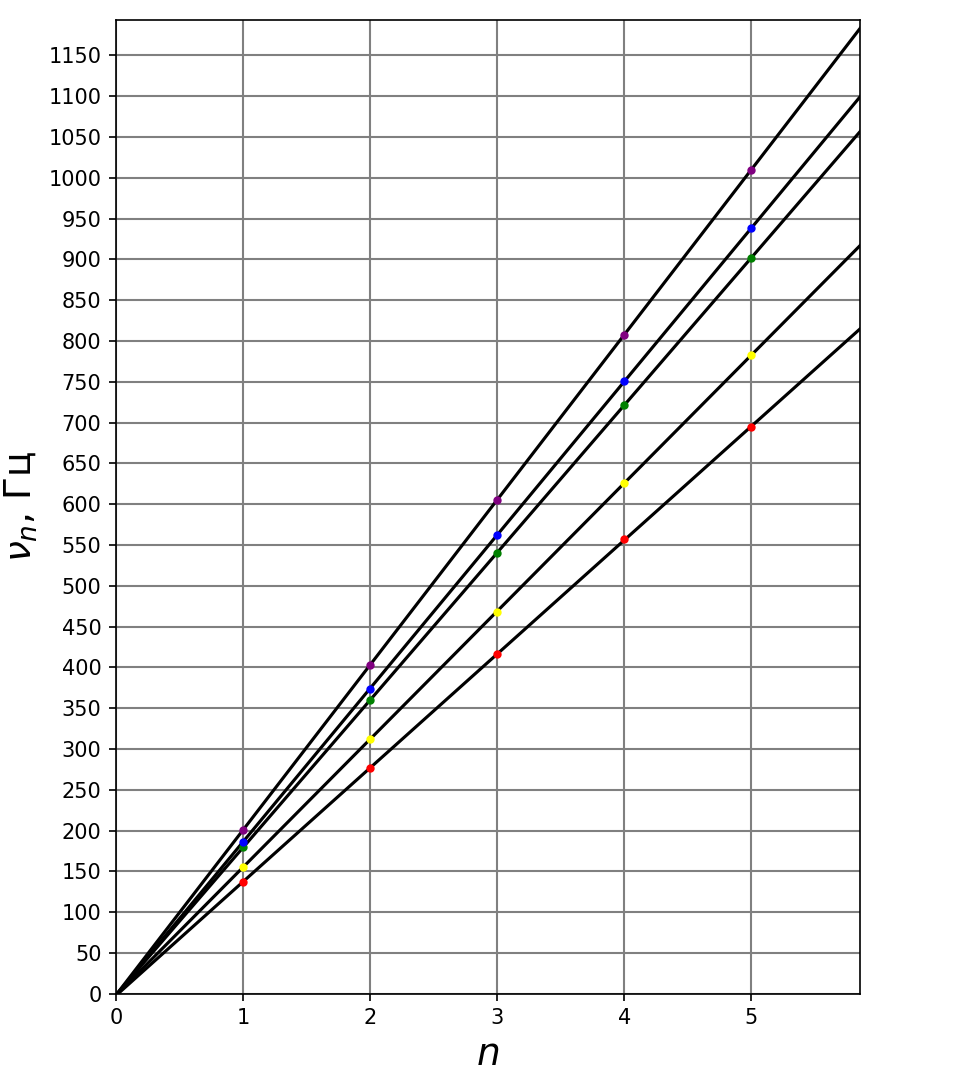
\includegraphics[scale=0.6]{Screenshot 2023-10-11 065731.png}
    \caption{Зависимость частоты $\nu_n$ от номера гармоники $n$.}
    \label{fig:enter-label}
\end{figure}

\pagebreak

По формуле $\nu_{n} = \frac{nu}{2l}$ можно догадаться, что коэффициент наклона прямой равен $\frac{u}{2l}$. Из полученных коэффициентов наклона вычислены скорости распространения волн $u$ и их погрешности. Результат записан в таблицу 3.

\begin{table}[!ht]
    \centering
    \caption{Результаты вычисления $u$}
    \begin{tabular}{|l|l|l|l|l|l|}
    \hline
        $\overline{u}$, м/с & 139,52 & 156,89 & 180,68 & 188,03 & 202,3 \\ \hline
        $\sigma_u$, м/с & 2,3 & 1,78 & 1,41 & 1,73 & 1,55 \\ \hline
        $\varepsilon_u$ & 0,016 & 0,011 & 0,008 & 0,009 & 0,008 \\ \hline
    \end{tabular}
\end{table}

\begin{figure}[h]
    \centering
    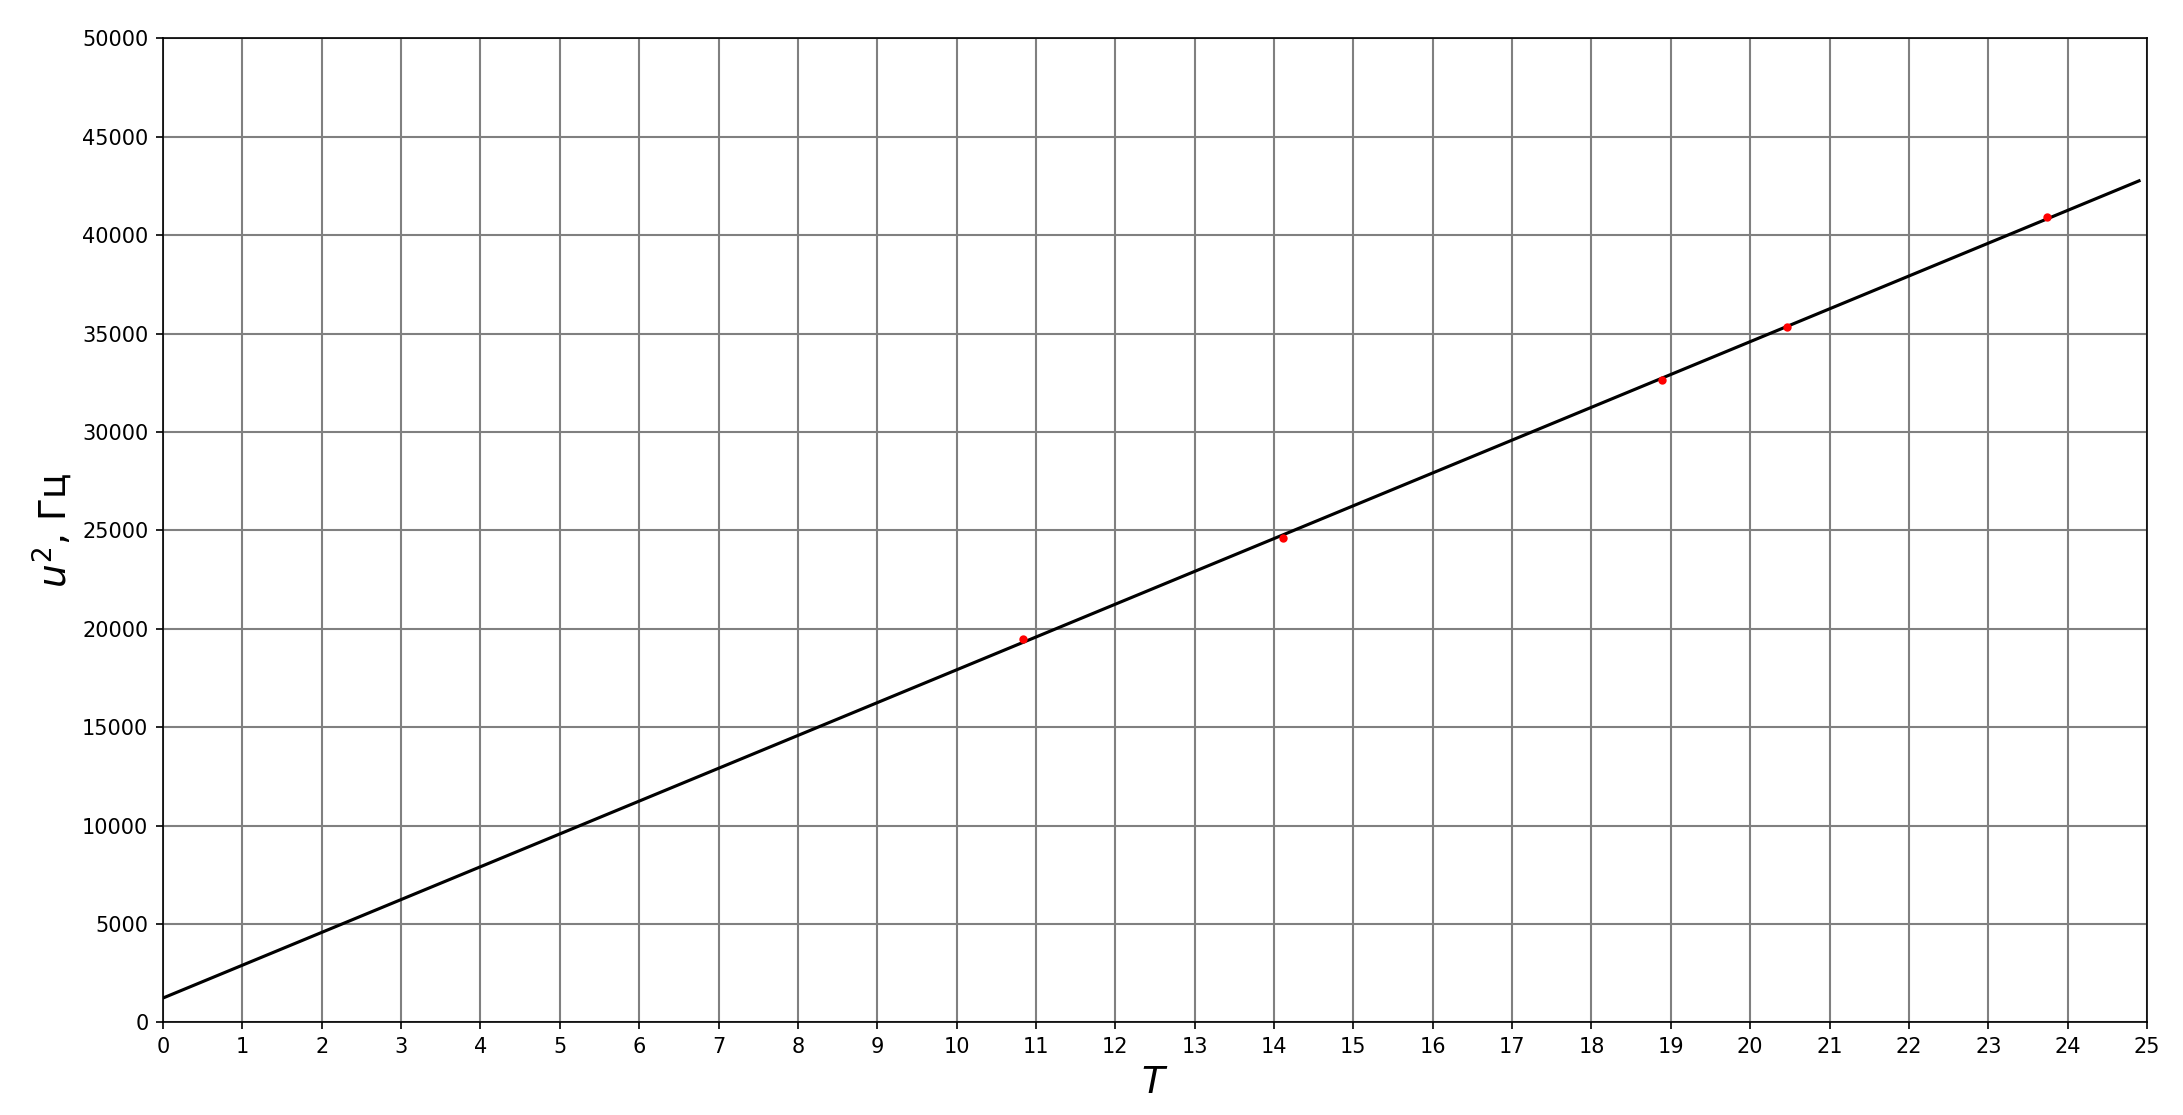
\includegraphics[scale=0.45]{Screenshot 2023-10-11 140253.png}
    \caption{График $u^2(T)$}
    \label{fig:enter-label}
\end{figure}

Угловой коэффициент посторенной по МНК аппроксимирующей прямой на рисунке 3 равен 1667,53, а также равен $\frac{1}{\rho_l}$. Следовательно $\rho_l$ = 599,69 мг/м. Относительная погрешность $\varepsilon_\rho$ = 0,01.

\section{Вывод}
В работе была экспериментально проверена зависимость $\nu_{n} = \frac{n}{2l}\sqrt{\frac{T}{\rho_l}}$, Результаты вычисления линейной плотности струны $\rho_l$ = 599,69 мг/м показывают, что, применяя данную формулу отклонение от реальной плотности струны (568,4 мг/м) составляет 5,5\%. 

\end{document}